\documentclass[12pt,titlepage]{article}
\usepackage[table]{xcolor}
\usepackage{longtable}
\usepackage[utf8]{inputenc}
%Language of Document Elements like Figure or Table
\usepackage[english]{babel}
\usepackage[bookmarks]{hyperref}
\usepackage{pdfpages}
\usepackage{graphicx}
\usepackage{float}
\usepackage{array}
\usepackage{lipsum} 
\usepackage[justification=centering]{caption}
\usepackage{enumitem}
\usepackage{chngcntr}
\usepackage{lscape}
\usepackage{fancyhdr}
\usepackage{listings}
\usepackage[style=alphabetic, backend=biber]{biblatex}
\usepackage{dafny}
\usepackage{hyperref}
\usepackage{nameref}
\usepackage[margin=1in]{geometry}

%Each Section in a new Page
\let\oldsection\section
\renewcommand\section{\clearpage\oldsection}

%Set space around and between lists
\setlist[enumerate]{noitemsep, topsep=0cm}
\setlist[itemize]{noitemsep, topsep=0cm}

%Figure/Table Numbering style "Section Number.figure counter
\renewcommand{\thefigure}{\arabic{section}.\arabic{figure}}
\renewcommand{\thetable}{\arabic{section}.\arabic{table}}

%Reset figure/table counter after section change
\counterwithin{figure}{section}
\counterwithin{table}{section}

%Syntax Highlighting
\lstdefinestyle{dafny}{language=dafny, frame=lr}

\colorlet{punct}{red!60!black}
\definecolor{background}{HTML}{EEEEEE}
\definecolor{delim}{RGB}{20,105,176}
\colorlet{numb}{magenta!60!black}

\lstdefinelanguage{json}{
	basicstyle=\normalfont\ttfamily,
	numbers=left,
	numberstyle=\scriptsize,
	stepnumber=1,
	numbersep=8pt,
	showstringspaces=false,
	breaklines=true,
	frame=lines,
	backgroundcolor=\color{background},
	literate=
	*{0}{{{\color{numb}0}}}{1}
	{1}{{{\color{numb}1}}}{1}
	{2}{{{\color{numb}2}}}{1}
	{3}{{{\color{numb}3}}}{1}
	{4}{{{\color{numb}4}}}{1}
	{5}{{{\color{numb}5}}}{1}
	{6}{{{\color{numb}6}}}{1}
	{7}{{{\color{numb}7}}}{1}
	{8}{{{\color{numb}8}}}{1}
	{9}{{{\color{numb}9}}}{1}
	{:}{{{\color{punct}{:}}}}{1}
	{,}{{{\color{punct}{,}}}}{1}
	{\{}{{{\color{delim}{\{}}}}{1}
	{\}}{{{\color{delim}{\}}}}}{1}
	{[}{{{\color{delim}{[}}}}{1}
	{]}{{{\color{delim}{]}}}}{1},
}


%TODO
\newcommand{\todonl}[1]{\newline\textcolor{red}{TODO: #1}\PackageWarning{TODO:}{#1!}}
\newcommand{\todo}[1]{\textcolor{red}{TODO: #1}\PackageWarning{TODO:}{#1!}}

%Set Paragraph indent to null
\setlength{\parindent}{0pt}
% Smaler Table Space
\renewcommand{\arraystretch}{1.5}

\title{Visual Studio Code Integration for the Dafny Language and Program Verifier}
\author{Rafael Krucker, Markus Schaden}
\date{20.02.2017}

\pagestyle{fancy}
\lhead{BA Dafny}
\addbibresource{LITERATURVERZEICHNIS/bibliographie.bib}
\begin{document}
\pagenumbering{Roman} 

% TODO
%
\includepdf{titlepage/titlepage}

% TODO
%\phantomsection
\addcontentsline{toc}{section}{Abstract}
\section*{Abstract}
[Placeholder Abstract Text]
%\newpage
%\phantomsection
\addcontentsline{toc}{section}{Management Summary}
\section*{Management Summary}
\subsection*{Ausgangslage}
[Placeholder]

\subsection*{Vorgehen}
[Placeholder]

\subsection*{Technologien}
[Placeholder]

\subsection*{Ergebnisse}
[Placeholder]

\subsection*{Ausblick}
[Placeholder]


% TODO
%\includepdf[pages={1-}, 
%scale=0.9,pagecommand=\thispagestyle{plain}]{additionals/eigenstaendigkeit}
%\includepdf[pages={1-2}, 
%scale=0.9,pagecommand=\thispagestyle{plain}]{additionals/aufgabenstellung}

\newpage
\tableofcontents
\newpage
\pagenumbering{arabic}
\section{Outline}
\subsection{The problem and its setting}
This chapter presents the background of the study, problem and its significance, and the scope and deliminition of the study.
\subsubsection{Introduction}
Dafny is a language designed and implemented by Microsoft Research. It offers built-in specification constructs. These include pre- and postconditions, frame specifications as well as termination metrics. Further support such as ghost variables and recursive functions are also implemented. Through such specification primitives, the Dafny verifier, invoked during compilation, can be used to verifiy the specified aspects of the functional correctness of the program. \newline
Dafny is typically used via its Visual Studio  IDE integration under the Windows operating system. Dafny can be run from the command line and a Visual Studio integration exists. The This integration verifier therefor allows for an efficient workflow of editing a program while constantly being given feedback about its the functional correctness. The Dafny compiler and verifier can additionally be invoked from the command line. \newline
Microsoft would like to integrate of Dafny into the cross-platform Visual Studio Code IDE. Work on this has already been started through a plugin by Jonathan  Rionatan. It currently works within the mono-environment and provides feedback from the verifier. \newline

\subsubsection{Statement of the problem}
This thesis aimes to research on how Dafny programmers can be best supported during their work and incorporate these findings in a production quality plugin for Visual Studio Code. 
\subsubsection{Significance of study}
Since the goal of the thesis is a production quality plugin, the thesis aims to immidiately simplify the way programmers use Dafny. Through Dafny's strong functional correctness facilities and Visual Studio Code's simple and modular architecture there is a chance that the plugin could guide developers through the transition to world of multi-core and multi-threaded applications, which are becoming more and more popular. Also in high risk domains the use of a specification constructs is of great benefit for the developers, which the developed plugin aims to make easier to harvest.
\subsubsection{Scope and delimination}
The plugin is limited to be used in three defined environments, although they compromise a huge percentage of environments used in programming. The plugin offers a fixed set of features which are detailed in this thesis, but remains open for adaption and extension.
\subsubsection{Definition of terms}

\section{Use Cases}
\subsection{Use Case Diagram}
\begin{figure}[h]
	\centering
	\includegraphics[width=1\linewidth, height=5in]{"./img/UseCase"}
	\caption{Use Case Diagram}
	\label{fig:usecase-diagram}
\end{figure}
\subsection{Actors and Stakeholder}
\begin{itemize}
	\item Programmers
	\item Microsoft
\end{itemize}
\subsection{Descriptions (brief)}
\subsubsection{UC1: Windows Installation}
A programmer can install the Dafny Plugin on his .Net environment running on Windows 10.
\subsubsection{UC2: Linux Installation}
A programmer can install the Dafny Plugin on his mono environment running on a common Linux distribution such as Ubuntu 16.04.
\subsubsection{UC3: OSX Installation}
A programmer can install the Dafny Plugin on his mono environment running on OSX ??? (VERSION).
\subsubsection{UC4: Easy installation of Dafny plugin}
A programmer can simply install the Dafny plugin by running an automatic installer which sets all path variables and makes additional needed environment adjustments.
\subsubsection{UC5: Syntax Highlighting}
The system automatically does syntax highlighting while the user writes a Dafny (dfy.) file.
\subsubsection{UC6: Reporting of Dafny best practices violations}
The plugin can be configured with a simple DSL config file which describes common best practices for Dafny. The plugin reports violations of these rules via the standard Visual Studio Code notification mechanisms.
\subsubsection{UC7: Automatic generation of contracts}
The plugin can be configured with a simple DSL-File to recognize certain semantics, which could benefit from the setting of Pre- and Postconditions. The plugin offers to add these in form of a refactoring via the common Visual Studio Code mechanisms.
\subsubsection{UC8: Autocompletion for identifiers}
The plugin offers autocompletion of Dafny code while the user types via the standard Visual Studio Code mechanisms.
\subsection{Descriptions (fully dressed)}
\subsubsection{UC1: Windows Installation}
\rowcolors{1}{gray!25}{white}
\begin{longtable}{l | p{0.7\textwidth} }
	Description & A programmer can install the Dafny Plugin on his .Net environment running on Windows 10.\\ \hline
	Primary Actor & Programmer\\ \hline
	Trigger & Programmer wants to programm Dafny in Visual Studio Code.\\ \hline
	Stakeholder and Interests & 
	\begin{itemize}
		\item Programmer: Wants stable support from the IDE while developing Code.
		\item Microsoft: Wants a stable Dafny integration to fulfill the needs of its clients.
	\end{itemize} \\ \hline
	Preconditions & 
 \begin{itemize}
		\item Windows 10 Environment with a modern version of the .Net Framework installed.
	\end{itemize} \\ \hline
	Postconditions & 
	\begin{itemize}
		\item The plugin works without problems, the programmer can start writing code.
	\end{itemize} \\ \hline
	Main Success Scenario & 1. Programmer downloads the plugin. \newline
	2. During an automated installation routine, the plugin installs itself and all needed environmental changes are made. (UC4) \newline
	3. Visual Studio code is updated to use the plugin, a success message is shown\\ \hline
	Extensions & 
	2a. The installer notices that some dependencies are missing. \newline 
	- It notifies the programmer accordingly.\\ \hline
	Special Requirements & None\\ \hline
	Frequency of Occurence & Usually once per working environment\\ \hline
	Open Issues & None \\ \hline
	\caption{UC1}
\end{longtable}
\subsubsection{UC2: Linux Installation}
\begin{longtable}{l | p{0.7\textwidth} }
	Description & A programmer can install the Dafny Plugin on his mono environment running on a common Linux distribution such as Ubuntu 16.04.\\ \hline
	Primary Actor & Programmer\\ \hline
	Trigger & Programmer wants to programm Dafny in Visual Studio Code.\\ \hline
	Stakeholder and Interests & 
	\begin{itemize}
		\item Programmer: Wants stable support from the IDE while developing Code.
		\item Microsoft: Wants a stable Dafny integration to fulfill the needs of its clients.
	\end{itemize} \\ \hline
	Preconditions & 
	\begin{itemize}
		\item A modern common Linux distribution such Ubuntu 16.04 or Fedora with the mono framework installed.
	\end{itemize} \\ \hline
	Postconditions &
	\begin{itemize}
		\item The plugin works without problems, the programmer can start writing code.
	\end{itemize} \\ \hline
	Main Success Scenario &
	1. Programmer downloads the plugin. \newline
	2. During an automated installation routine, the plugin installs itself and all needed environmental changes are made. (UC4) \newline
	3. Visual Studio code is updated to use the plugin, a success message is shown\\ \hline
	Extensions &
	2a. The installer notices that some dependencies are missing. \newline
	- It notifies the programmer accordingly.\\ \hline
	Special Requirements & None\\ \hline
	Frequency of Occurence & Usually once per working environment\\ \hline
	Open Issues & None \\ \hline
	\caption{UC2}
\end{longtable}

\subsubsection{UC3: OSX Installation}
\begin{longtable}{l | p{0.7\textwidth} }
	Description & A programmer can install the Dafny Plugin on his mono environment running on OSX.\\ \hline
	Primary Actor & Programmer\\ \hline
	Trigger & Programmer wants to programm Dafny in Visual Studio Code.\\ \hline
	Stakeholder and Interests & 
	\begin{itemize}
		\item Programmer: Wants stable support from the IDE while developing Code.
		\item Microsoft: Wants a stable Dafny integration to fulfill the needs of its clients.
	\end{itemize} \\ \hline
	Preconditions &
	\begin{itemize}
		\item A modern version of the OSX OS installed such as canberra with the mono framework installed.
	\end{itemize} \\ \hline
	Postconditions &
	\begin{itemize}
		\item The plugin works without problems, the programmer can start writing code.
	\end{itemize} \\ \hline
	Main Success Scenario & 1. Programmer downloads the plugin. \newline
	2. During an automated installation routine, the plugin installs itself and all needed environmental changes are made. (UC4) \newline
	3. Visual Studio code is updated to use the plugin, a success message is shown\\ \hline
	Extensions & 
	2a. The installer notices that some dependencies are missing. \newline 
	- It notifies the programmer accordingly.\\ \hline
	Special Requirements & None\\ \hline
	Frequency of Occurence & Usually once per working environment\\ \hline
	Open Issues & None \\ \hline
	\caption{UC3}
\end{longtable}

\subsubsection{UC4: Easy installation of Dafny plugin}
\begin{longtable}{l | p{0.7\textwidth} }
	Description & A programmer can simply install the Dafny plugin by running an automatic installer which sets all path variables and makes additional needed environment adjustments.\\ \hline
	Primary Actor & Programmer\\ \hline
	Trigger & Programmer wants install the Dafny plugin to visual studio code.\\ \hline
	Stakeholder and Interests & Programmer: Wants an easy, automated installation of the plugin. \newline Microsoft: Wants a stable Dafny integration to fulfill the needs of its clients.\\ \hline
	Preconditions &\begin{itemize}
		\item Depending on the environment, the preconditions of UC1, UC2 or UC3 are satisfied.
		\item Visual Studio Code is installed.
		\item The programmer has admin priviledges in his environment.
	\end{itemize}\\ \hline
	Postconditions & 
	\begin{itemize}
		\item The plugin works without problems, the programmer can start writing code.
	\end{itemize} \\ \hline
	Main Success Scenario & 
	1. Programmer downloads the plugin via the Visual Studio Code plugin store. \newline
	2. The plugin determines which platform it is run on, and sets either the path to the .Net framework or the mono framework. \newline
	3. The plugin downloads the Dafny and sets the path to the Dafny server binary. \newline
	4. The plugin then installs itself via the standard Visual Studion Code plugin mechanisms. \newline
	5. The plugin prompts a success message and the programmer is ready to code in Dafny.\\ \hline
	Extensions & 
	2a. The installer can't find, depending on the enviroment, either the mono or the .Net framework in the standard locations. \newline 
	- It prompts the user to enter the location and does so until the framework is found. \\ \hline
	Special Requirements & None\\ \hline
	Frequency of Occurence & Usually once per working environment\\ \hline
	Open Issues & None \\ \hline
	\caption{UC4}
\end{longtable}

\subsubsection{UC5: Syntax Highlighting}
\begin{longtable}{l | p{0.7\textwidth} }
	Description & The system automatically does syntax highlighting while the user writes a Dafny (dfy.) file.\\ \hline
	Primary Actor & Programmer\\ \hline
	Trigger & Programmer writes Dafny code in Visual Studio Code.\\ \hline
	Stakeholder and Interests & Programmer: Wants enhanced readability for the source files he's working on. \newline Microsoft: Wants a state of the art IDE integration of Dafny.\\ \hline
	Preconditions &
	\begin{itemize}
		\item Visual Studio Code with the Dafny plugin installed is running.
		\item Dafny code is being written in a .dfy file.
	\end{itemize}\\ \hline
	Postconditions &
	\begin{itemize}
		\item The source code is highlighted in different colors according to common standards in general and the Visiual Studio Code guidelines specifically.
	\end{itemize}\\ \hline
	Main Success Scenario & 
	1. Programmer types code into a .dfy file. \newline
	2. The plugin detects the changes and applies syntax highighlighting through the standard Visual Studio Code mechanisms.\\ \hline
	Extensions & 
	2a. The newly written code causes a compilation error and cannot be interpreted. \newline 
	- The previous syntax highlighting stays in place, the errors are highlighted according to common practices with compilation errors in Visual Studio Code. \\ \hline
	Special Requirements & None\\ \hline
	Frequency of Occurence & Very often, after every key up event.\\ \hline
	Open Issues & None \\ \hline
	\caption{UC5}
\end{longtable}

\subsubsection{UC6: Reporting of Dafny best practices violations}
\begin{longtable}{l | p{0.7\textwidth} }
	Description & The plugin can be configured with a simple DSL config file which describes common best practices for Dafny. The Plugin reports violations of these rules via the standard Visual Studio Code notification mechanisms.\\ \hline
	Primary Actor & Programmer\\ \hline
	Trigger & Programmer writes Dafny code in Visual Studio Code.\\ \hline
	Stakeholder and Interests & Programmer: Wants to write the cleanest code possible using common Dafny idioms. \newline Microsoft: Wants to support programmers getting the most out of Dafny.\\ \hline
	Preconditions &
	\begin{itemize}
		\item Visual Studio Code with the Dafny plugin installed is running.
		\item Dafny code is being written in a .dfy file.
	\end{itemize}\\ \hline
	Postconditions &
	\begin{itemize}
		\item Violations of common best practices for Dafny are reported through the standard Visual Studio Code mechanisms.
	\end{itemize}\\ \hline
	Main Success Scenario & 
	1. The plugin is installed preconfigured with a collection of common best practives for Dafny, which is done through a DSL file. \newline
	2. Programmer types code into a .dfy file. \newline 
	3. The plugin continuously checks for violations of the rules. \newline 
	4. If a violation is detected, it is reported through the standard mechanisms of Visual Studio Code.\\ \hline
	Extensions & 
	1a. The predefined rules are not sufficient for the programmer. \newline 
	- The programmer can updated the configuration file himself to include his own or his company's coding guidelines. \\ \hline
	Special Requirements & None\\ \hline
	Frequency of Occurence & Very often, after new valid syntax was written.\\ \hline
	Open Issues & None \\ \hline
	\caption{UC6}
\end{longtable}

\subsubsection{UC7: Automatic generation of contracts}
\begin{longtable}{l | p{0.7\textwidth} }
	Description & The plugin can be configured with a simple DSL-File to recognize certain semantics, which could benefit from the setting of Pre- and Postconditions. The plugin offers to add these in form of a refactoring via the common Visual Studio Code mechanisms.\\ \hline
	Primary Actor & Programmer\\ \hline
	Trigger & Programmer writes Dafny code in Visual Studio Code.\\ \hline
	Stakeholder and Interests & Programmer: Wants to write the correctest code possible making use of Dafny's specification constructs. \newline Microsoft: Wants to support programmers getting the most out of Dafny.\\ \hline
	Preconditions &
	\begin{itemize}
		\item Visual Studio Code with the Dafny plugin installed is running.
		\item Dafny code is being written in a .dfy file.
	\end{itemize}\\ \hline
	Postconditions &
	\begin{itemize}
		\item Specification constructs suitable for the context were added as refactorings.
	\end{itemize}\\ \hline
	Main Success Scenario & 
	1. The plugin is installed preconfigured with a collection of common semantics for Dafny and their corresponding specification constraints, which is done through a DSL file. \newline
	2. Programmer types code into a .dfy file. \newline 
	3. The plugin continuously checks for semantics that could benefit form the setting of specification constraints. \newline 
	4. If such a semantic is detected, it is reported through the standard mechanisms of Visual Studio Code, with a refactoring offered to add the constraints. \newline
	5. The programmer invokes the refactorings and the necessary code is added.\\ \hline
	Extensions & 
	1a. The predefined semantics and refactorings are not sufficient for the programmer. \newline 
	- The programmer can updated the configuration file himself to include support for his own or his company's  common code semantics. \\ \hline
	Special Requirements & None\\ \hline
	Frequency of Occurence & Very often, after new valid syntax was written.\\ \hline
	Open Issues & None \\ \hline
	\caption{UC7}
\end{longtable}

\subsubsection{UC8: Autocompletion for identifiers}
\begin{longtable}{l | p{0.7\textwidth} }
	Description & The plugin offers autocompletion of Dafny code while the user types via the standard Visual Studio Code mechanisms.\\ \hline
	Primary Actor & Programmer\\ \hline
	Trigger & Programmer writes Dafny code in Visual Studio Code.\\ \hline
	Stakeholder and Interests & Programmer: Wants enhanced productivity while writing Dafny code. \newline Microsoft: Wants a state of the art IDE integration of Dafny.\\ \hline
	Preconditions &
	\begin{itemize}
		\item Visual Studio Code with the Dafny plugin installed is running.
		\item Dafny code is being written in a .dfy file.
	\end{itemize}\\ \hline
	Postconditions &
	\begin{itemize}
		\item An identifier was autocompleted.
	\end{itemize}\\ \hline
	Main Success Scenario & 
	1. Programmer types code into a .dfy file. \newline
	2. The plugin detects the changes and searches for the beginning of known identifiers. \newline
	3. If such a beginning is found, completion if offered through the standard mechanisms of Visual Studio Code.\\ \hline
	Extensions & 
	None. \\ \hline
	Special Requirements & None\\ \hline
	Frequency of Occurence & Very often, after every key up event.\\ \hline
	Open Issues & None \\ \hline
	\caption{UC8}
\end{longtable}
\section{Project management}
\subsection{Projectplan}
\begin{figure}[H]
	\centering
	\includegraphics[width=1.2\textwidth]{img/projectplan}
	\caption{Projectplan}
	\label{fig:Projectplan}
\end{figure}
\subsection{Milestones}
\rowcolors{1}{gray!25}{white}
\begin{longtable}[H]
	{l| l | p {0.7\textwidth}}
	\textbf{Nr} & \textbf{Title} & \textbf{Description} \\ 
	\hline\hline
	
	M1 & First prototype & Plugin is working on all operation systems, simple verification is in place and errors are reported, basic syntax highlighting \\ 
	
	M2 & Improved prototype & Automatic downloading of dependencies and installation of Dafny and configure of environment variables \\ 
	
	M3 & Contract generation & First automatic contract generation, customizable with DSL \\ 
	
	M4 & Autocompletion & Autocompletion for identifiers \\ 
	
	M5 & Release 1.0 & Everything implemented and tested. Ready to be published \\ 		
	\caption{Milestone}
	\label{tab:Milestone}
\end{longtable}
\subsection{Risk management}
\begin{landscape}
	\rowcolors{2}{gray!25}{white}
	\begin{longtable}[H]
		{l|p{0.22\textwidth}| p{0.22\textwidth} | p{0.1\textwidth} | p{0.1\textwidth} | p{0.25\textwidth} | p{0.25\textwidth}}
		
		\textbf{Nr} & \textbf{Title} & \textbf{Description} & 
		\textbf{Max Harm [h]} & \textbf{Proba- bility} & \textbf{Prevention} &  
		\textbf{Behaviour at entry}\\ \hline
		
		R1 & Underestimation of workload & One or more team members can't finish a feature in time or loses to much time on a minor feature & 120 & 25\% & Weekly scrum meetings with feedback about the current work progress. Estimate workload together. Include time reserve & Help each other, if one is struggling. Feature reduction as last resort. \\ 
		
		R2 & Workflow is not working & Toolchain is not working as planed. The used components aren't ideal for the problem & 30 & 15\% & Use experience to get a good setup and test it alot in the beginning & Redefine toolchain or change single tool \\ 
		
		R3 & Communication problems & Team is not working together and each member is developing individually. Creation of incompatible interfaces. Talking with the industrial partner isn't possible as expected, due to time difference or not enough time & 70 & 20\% & Weekly scrum meetings and agreements. Already worked in other projects as a team before & Increase written documentation and working closer together. Having a fixed meeting with the industrial partner \\ 
		
		R4 & Lack of knowledge & Team has to little knowledge about Dafny, VSCode and the development of a VSCode Plugin & 80 & 10\% & Already experience with typescript for plugin development, as preparatory work informed about Dafny & Find necessary knowledge online, get help from Microsoft Research \\ 
		
		R5 & Data loss or manipulation & Data loss because of a server crash or open permissions to access and modify data & 20 & 3\% & Regularly backups and restrictive permissions to change files & Use backup to restore data. Extend safety measures \\ 
		
		R6 & Failure developer machine & One of the developer machines isn't working anymore. & 10 & 1\% & Limited, regularly commits and backups. & Switch temporary to the school computer and install the necessary tools. \\
		
		R7 & Implementing the DSL is too complicated or too difficult to use & The DSL would be needed to suggest possible contracts or to customize the best practices. & 100 & 30\% & This core feature has to be researched carefully so that it really fits our needs and that other developers can really use the plugin. & Read about DSL, talking to people which have already worked with it. \\
		
		R8 & Supporting all features on the different environments is not possible & Due to that Windows, OSX and Linux are quite different, it could be that some features aren't possible to implement on a platform or causes a big overhead to get it running & 10 & 25\% & Using as much of the standard API as possible. Implement specific features platform dependant. & Disable a certain feature on a platform or look for a workaround. \\	
		
		R9 & Automatic installer of Dafny is not possible & Maybe because of security restrictions, it could be possible that you can't download and install additional software and set environment variables. & 35 & 20\% & Test if downloading of software can done inside VS Code. & Automatic installer can't be done inside the plugin. Switch to a different strategy and implement an automatic installer over a additional executable, which could also install the plugin in vscode. \\
		
		\caption{Risk management}
		\label{tab:Risk management}
	\end{longtable}
\end{landscape}

\subsection{Risk Matrix}
\begin{figure}[H]
	\centering
	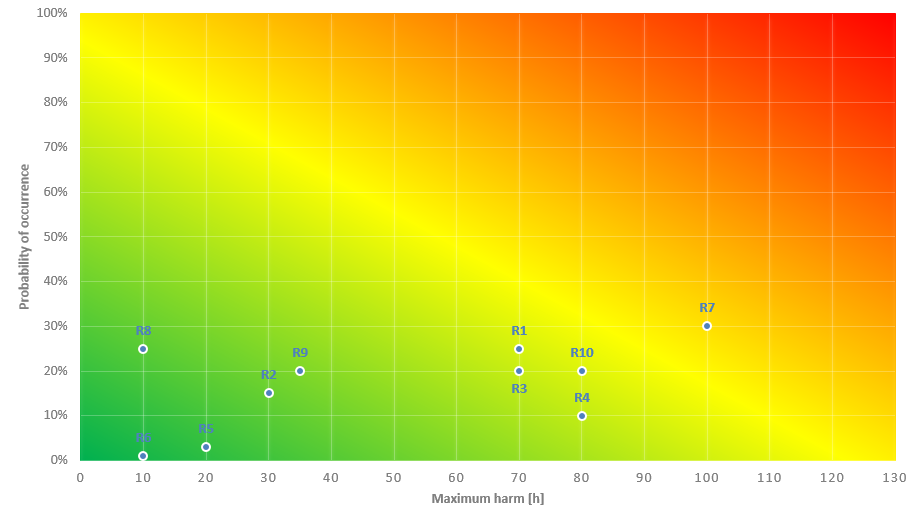
\includegraphics[width=1\textwidth]{img/riskmatrix}
	\caption{Risk Matrix}
	\label{fig:Risk Maxtrix}
\end{figure}
\section{Systemsetup}
\subsection{Local setup}
TexStudio 2.12\newline
Visual Studio Code 1.9\newline
Git 


\subsection{Server setup}
Jira \newline
Bamboo\newline
NodeJS\newline
SonarQube\newline
Postgres


\subsection{Continuous Integration}

To ensure that the code quality is high and the code is working as expected, all commits trigger automated builds of the respective project. A commit to the documentation repository executes a job which creates a pdf out of the latex sources. This document is then copied to the wwwroot directory, which then can be downloaded from the project homepage. Commits to the vscode-dafny repository will result in a build and a complete run of all tests on the three environments afterwards. Therefore remote agents are installed on Ubuntu and OSX , which test the plugin on these operation system.  Additionally SonarQube is used to find bugs and bad pratices as early as possible. The last repository which triggers a bamboo job is the project homepage. The latest version is built and deployed when a commit happens. 


\begin{figure}[H]
	\centering
	\includegraphics[width=1\textwidth]{img/ci}
	\caption{Server Setup}
	\label{fig:Server setup}
\end{figure}
\section{Conception and Design}
This chapter documents the most important design decisions and the rationale behind them.


\subsection{Contract generation examples} \label{examples}
Since Dafny offers built-in specification constructs, a programmer would greatly benefit from generation of contracts for common situations. This chapter first introduces three examples in programming, that could be made safer through the use of contracts. The solution is then generalized in order to be more widely applicable.
\subsubsection{Example 1: Array access} \label{Example 1}

\paragraph{Problem:}

A method access an array with an index, which is given as a parameter. The array may be a field or also be a parameter. The array may be null or the index may be out of bound.
\paragraph{Solution:}
Generate a precondition which checks if the array is not null and the index is in bound of the array.

\paragraph{Code:}
\begin{lstlisting}[language=dafny]
method FindUsafe(a: array<int>, key: int) return (element: int)
{
	return a[key];
}

method FindSafe(a: array<int>, key: int) return (element: int)
	requires a != null && 0 <= key < a.Length
{
	return a[key];
}
\end{lstlisting}



\subsubsection{Example 2: Simple domain specific constraints} \label{Example 2}
\paragraph{Problem:}
A method that processes withdraws form a bank account may not make a bank balance negative.
\paragraph{Solution:}
Generate a pre- and postconditions on methods which modify relevant fields, according to domain specific constraints.

\paragraph{Code:}
\begin{lstlisting}[language=dafny]
class BankAccountUnsafe {
	var balance: int;
	
	method withdraw(amount: int) modifies this {
		balance := balance - amount;
	}
}

class BankAccountSafe {
	var balance: int;
	
	method withdraw(amount: int) 
		requires balance >= amount  
		ensures balance >= 0  
	modifies this {
		balance := balance - amount;
	}
}
\end{lstlisting}


\subsubsection{Example 3: More complex Domain specific constraints} \label{Example 3}
\paragraph{Problem:}
A factory wants to model its processes. Their services consist of refining certain rawmaterials, which can interact aggressively with their machines. They have two types of machines, some which are subject to abreason over time, but also others which are very expensive and should not come into contact with aggressive materials. They want to make sure no aggressive materials come in contact with expensive machines under any circumstances.
\paragraph{Solution:}
Generate a pre- and postconditions on methods which modify relevant fields, according to domain specific constraints.

\paragraph{Code:}
\begin{lstlisting}[language=dafny]

class RawMaterial {
	var abreasesMachines: bool;
}

class NormalMachine {
	var prestine: bool;
	constructor() modifies this {
		this.prestine := true;
	}
	method refineMatieral(material: RawMaterial) {
		...
	}
	method processMaterial(material: RawMaterial) 
		requires material != null
	modifies this {
		this.refineMatieral(material);
		this.prestine := !material.abreasesMachines;
	}
}

class ExpensiveMachine {
	var prestine: bool;
	constructor() modifies this {
		this.prestine := true;
	}
	
	method refineMatieral(material: RawMaterial) {
	
	}
	
	method processMaterial(material: RawMaterial) 
		requires material != null
		requires !material.abreasesMachines
		ensures prestine
	modifies this {
		this.refineMatieral(material);
		this.prestine := !material.abreasesMachines;
	}
}
\end{lstlisting}

\subsubsection{Underlying problems}
All three examples have in common, that without the correct preconditions they should result in proof obligations which cannot be proven.
This subsection first details three common concepts that occur when reasoning about proof obligations. The next subsections sets them into connections with the problems mentioned in \ref{examples}.

\paragraph{Application of partial functions} \label{partial function}
One of the three problems can be expressed as the application of partial functions, which are defined by the following three objects:
\begin{itemize}
	\item A set A called the input set of the function
	\item A set B called the output set of the function.
	\item A rule f that transforms some elements of A to some elements of B such that no element a from A is transformed to more than one element of B.\cite[197]{khoussainov}
\end{itemize}
The definition states that not all input values may be mapped by the function. The problem here therefor is to ensure that the function is applied on only a valid subset of A.


\paragraph{Invariants} \label{invariants}
An Invariant can be defined as follows: A quantity which remains unchanged under certain classes of transformations. Invariants are extremely useful for classifying mathematical objects because they usually reflect intrinsic properties of the object of study.\cite[282ff]{hunt}
\newline An Invarant is therefor extremly useful when one wants to ensure certain conditions of an object, which must hold at all times. If an invariant is to be applied to an object with multiple attributes, it is usually defined as a postconditions on all attributes. 

\paragraph{Non provable Goals} \label{non provable goal}
These are situations, that are impossible to prove, because some preconditions do not hold or not sufficent information is available. They are very hard to detect and isolate from provable goals, although some work has found solutions under certain restrictions, for instance \cite{goals}. When an unprovable goal is encountered in a context, it is much easier to simply state it as a precondition for the context to be valid, thus burdening the calling context with ensuring that the goal holds. 

\subsubsection{Solving the problems in an abstract way}
This subsection finally shows how the patterns detailed above can be used to solve the programming examples, thus allowing generic solutions for many similar problems.

\paragraph{Problem 1}
The situation shown in \ref{Example 1} is a very common sitatuation while programming, basically one wants to prove that the index is always in the bounds of the array. Accessing an element in an array is an example of the \nameref{partial function}, where the set A only goes from zero to the length of the array minus one. Therefor one would have to prove that the application of the partial function does not result in an invalid element being given as an argument. The expression, which is used to get access can be arbitrarily complex. The computation to ensure the in-boundness can be very expensive.  \newline
Also the second pattern discussed in \nameref{invariants} could be applied, always ensuring that a given parameter is in bound of an array of an object, although this would not work with how invariants are normally applied, namely as postconditions. Since the expression that generates the index has nothing to do with the object itself, it is questionable if this is the right pattern to apply in this situation. \newline
The third pattern, discussesd in \nameref{non provable goal}, works very well if one assumes that it can't be proven that the expression will always lead to a successful application of the partial function (although it could be proven in many cases). This allows to define this property as a precondition of the method, thus shifting the burden to the caller to always check his arguments. this is an easy and feasable solution to the first problem. 

\paragraph{Problem 2} \label{Problem 2}
The example in \ref{Example 2} is an example of a domain specific limitation where a bankaccounts balance should never fall below zero. In this specific implementation the usage of \nameref{partial function} could be discussed, since it is implemented as binary minus function which only allows subtrahends from a certain range, although this approach could not be used for all possible implementations and is therefor not a feasable solution. \newline
The second pattern discussed in \nameref{invariants} best describes the semantics of the situation in a very general way, it could simply be stated as an Invariant, that the balance has always to be positive. This does not suffice though, as it does not isolate the parts yet which could break the invariant. \newline
The third pattern, discussesd in \nameref{non provable goal}, works very well in conjunction with the second one. All sub goals that should hold that the invariant holds, in this case that the amount should be smaller than the balance, can be viewed as unprovable goals in this context. They can be therefor be formulated as preconditions such that the caller has the burden of applying correct arguments to the function. This practice isolates the parts which could break the invariant, allowing to write the function as safe as possible.

\paragraph{Problem 3}
The example in \ref{Example 3} is also an example of a domain specific limitation, although more complex. It combines several classes together, which could also potentially be subtyped. The goal is to never let an expensive machine be subjected to abreason, therefore only allowing non-aggressive rawmaterials as input. In this specific implementation the usage of \nameref{partial function} could work very well, since the input set of the partial function is very small, namely only the value true on the abreasesMachines property of a rawmaterial. However, if we extend the hierarchy of materials and implement the calculation of abreasesMachines differently, it is unclear if all cases could be computet efficiently. \newline
The second pattern discussed in \nameref{invariants} best describes the semantics of the situation in a very general way, it could simply be stated as an Invariant, that the prestine property on the expensive machine is always true. This does not suffice though, as it does not isolate the parts yet which could break the invariant. This is the same situation as in \nameref{Problem 2} \newline
The third pattern could be much in the same way as in \nameref{Problem 2}. The condition, that the raw material may never abrease machines, can be written as a preconditions and together with the usage of invariants holds the greates amount of security regarding the domain constraints.

\subsubsection{Conclusion}
As the discussion above shows, all of the three problems can be solved through the application of \nameref{invariants} and \nameref{non provable goal}. They make it unnecessary to solve the problems of \nameref{partial function}, which is often harder to do. All occurences where such a computation would be needed can be seen as non provable goals and stated as preconditions for a method. The usage of invariants offers a syntactical  transparent way of describing domain specific rules, and the implementation is a relativ simple one, as it just is translated into postconditions for all methods of an object. Together these two techniques offer solutions to many different problems in computer science, since they operate on a high abstraction while still being syntactical transparent.\newline 
In the first example, the language itself has enough domain knowledge in order to generate the unprovable proof obligations by itself, since it knows about the array type and its restrictions. In the two other cases the language  needs more domain knowledge in order to generate the unprovable proof obligations. As was shown above, invariants are a good way of providing this domain knowledge.
Once the unprovable proof obgligations can be found, they can be used as hints for preconditions that can be suggested to the programmer.\newline
The hardest part of the implementation is the identification of non provable subgoals that are in relation to an invariant. To do this, detailed knowledge has to be available of the control flow of a program and all possible outcomes of a computation have to be considered, although the problem can be relaxed if one allows for false positives in the identification of non provable subgoals. Since the plugin only offers refactorings and does not apply them automatically, the programmer still can decide if the setting of the non provable goal as precondition is necessary.  


\subsection{Test specification}

\subsubsection{Integration Tests}
VS Code extensions that use the VS Code API can be tested with help of a special instance of VS Code. Inside this instance, the extension can use the full API and tests can execute commands like create a new file, enter a character, use the auto-complete and verify if the extension works as expected. Therefore  


\subsubsection{Unit Tests}
	Visual Studio Code plugins can be additionally tested with standard javascript testing frameworks like Mocha or Jasmine. This allows to test core logic without the need to run tests inside VS Code. 

\subsubsection{Testcases}

\begin{longtable}{ p{0.4\textwidth} | p{0.6\textwidth} }
	\textbf{Testcase} & \textbf{Verify}\\
	UC1: Windows Installation\newline 
	UC2: Linux Installation\newline 
	UC3: OSX Installation & 
		The language dafny is available\newline 
		.dfy files are associated with the dafny plugin\newline
		The server is started\newline
		The status is changed after the file have been checked\newline
		If the server crashes, this is reported and the server is restarted
	\\
	UC4: Easy installation of Dafny plugin & 
		The plugin automatically downloads and installs dafny\newline
		Sets the dafny server path \newline
		Shows a message if .Net framework or mono is missing
	\\
	UC5: Syntax Highlighting & 
		Syntax is highlighted
	\\
	UC6: Reporting of Dafny best practices violations &
		\todo{?}
	
 	\\
	UC7: Automatic generation of contracts & \todo{Invariant: Require and ensures are generated?} \\
	UC8: Autocompletion for identifiers & 
		Autocompletion is working for all known dafny identifiers\newline
		Methods are considered for autocompletion as well
		
	
	\\
\end{longtable}


%\section{Ergebnisse}
[Placeholder]
%\section{Ausblick}
[Placeholder]

\appendix

\listoffigures
\addcontentsline{toc}{section}{\listfigurename}

\listoftables
\addcontentsline{toc}{section}{\listtablename}
\printbibliography[heading=bibintoc]
%\section{Anhang}
[Placeholder]
\end{document}
